% ----------------------------------------------------------------- %
%             The Speech Signal Processing Toolkit (SPTK)           %
%             developed by SPTK Working Group                       %
%             http://sp-tk.sourceforge.net/                         %
% ----------------------------------------------------------------- %
%                                                                   %
%  Copyright (c) 1984-2007  Tokyo Institute of Technology           %
%                           Interdisciplinary Graduate School of    %
%                           Science and Engineering                 %
%                                                                   %
%                1996-2016  Nagoya Institute of Technology          %
%                           Department of Computer Science          %
%                                                                   %
% All rights reserved.                                              %
%                                                                   %
% Redistribution and use in source and binary forms, with or        %
% without modification, are permitted provided that the following   %
% conditions are met:                                               %
%                                                                   %
% - Redistributions of source code must retain the above copyright  %
%   notice, this list of conditions and the following disclaimer.   %
% - Redistributions in binary form must reproduce the above         %
%   copyright notice, this list of conditions and the following     %
%   disclaimer in the documentation and/or other materials provided %
%   with the distribution.                                          %
% - Neither the name of the SPTK working group nor the names of its %
%   contributors may be used to endorse or promote products derived %
%   from this software without specific prior written permission.   %
%                                                                   %
% THIS SOFTWARE IS PROVIDED BY THE COPYRIGHT HOLDERS AND            %
% CONTRIBUTORS "AS IS" AND ANY EXPRESS OR IMPLIED WARRANTIES,       %
% INCLUDING, BUT NOT LIMITED TO, THE IMPLIED WARRANTIES OF          %
% MERCHANTABILITY AND FITNESS FOR A PARTICULAR PURPOSE ARE          %
% DISCLAIMED. IN NO EVENT SHALL THE COPYRIGHT OWNER OR CONTRIBUTORS %
% BE LIABLE FOR ANY DIRECT, INDIRECT, INCIDENTAL, SPECIAL,          %
% EXEMPLARY, OR CONSEQUENTIAL DAMAGES (INCLUDING, BUT NOT LIMITED   %
% TO, PROCUREMENT OF SUBSTITUTE GOODS OR SERVICES; LOSS OF USE,     %
% DATA, OR PROFITS; OR BUSINESS INTERRUPTION) HOWEVER CAUSED AND ON %
% ANY THEORY OF LIABILITY, WHETHER IN CONTRACT, STRICT LIABILITY,   %
% OR TORT (INCLUDING NEGLIGENCE OR OTHERWISE) ARISING IN ANY WAY    %
% OUT OF THE USE OF THIS SOFTWARE, EVEN IF ADVISED OF THE           %
% POSSIBILITY OF SUCH DAMAGE.                                       %
% ----------------------------------------------------------------- %
\hypertarget{window}{}
\name{window}{data windowing}{signal processing,speech analysis and synthesis}

\begin{synopsis}
\item[window] [ --l $L_1$ ] [ --L $L_2$] [ --n $N$ ] [ --w $W$ ] [ {\em infile} ]
\end{synopsis}

\begin{qsection}{DESCRIPTION}
{\em window} multiplies, 
on an element-by-element basis, 
length $L$ input vectors from {\em infile} (or standard input) 
by a specified windowing function, 
sending the result to standard output.

For the input data
\begin{displaymath}
  x(0), x(1), \dots, x(L_1-1)
\end{displaymath}
and the windowing function
\begin{displaymath}
  w(0), w(1), \dots, w(L_1-1), 
\end{displaymath}
the output is calculated as follows:
\begin{displaymath}
  x(0)\cdot w(0),\,x(1)\cdot w(1),\,\dots,\,x(L_1-1)\cdot w(L_1-1). 
\end{displaymath}
If $L_2$ is greater then $L_1$, then 0s are added to the output as follows.
\begin{displaymath}
  \underbrace{x(0)\cdot w(0),\,x(1)\cdot w(1),\,\dots,\,x(L_1-1)\cdot w(L_1-1),0,\dots,0}_{L_2}
\end{displaymath}

Input and output data are in float format.
\end{qsection}

\begin{options}
	\argm{l}{L_1}{frame length of input $(L\leq 2048)$}{256}
	\argm{L}{L_2}{frame length of output}{$L_1$}
	\argm{n}{N}{type of normalization\\
			\begin{tabular}{ll}\\ [-1ex]
			 0 & no normalization\\
			 1 & normalization as
                             $\displaystyle \sum_{n=0}^{L-1} w^2(n) = 1$\\
			 2 & normalization as
                             $\displaystyle \sum_{n=0}^{L-1} w(n) = 1$\\
			 \end{tabular}\\\hspace*{\fill}}{1}
	\argm{w}{W}{type of window\\
			\begin{tabular}{ll}\\ [-1ex]
			 0 & Blackman \\
			 1 & Hamming \\
			 2 & Hanning \\
			 3 & Bartlett \\
			 4 & trapezoid \\
			 5 & rectangular \\
			\end{tabular}\\\hspace*{\fill}}{0}
\end{options}

\begin{qsection}{EXAMPLE}
This example prints in the screen a sin wave function
with period 20 after windowing it with a Blackman window:
\begin{quote}
  \verb!sin -p 20 | window | fdrw | xgr !
\end{quote}
\begin{center}
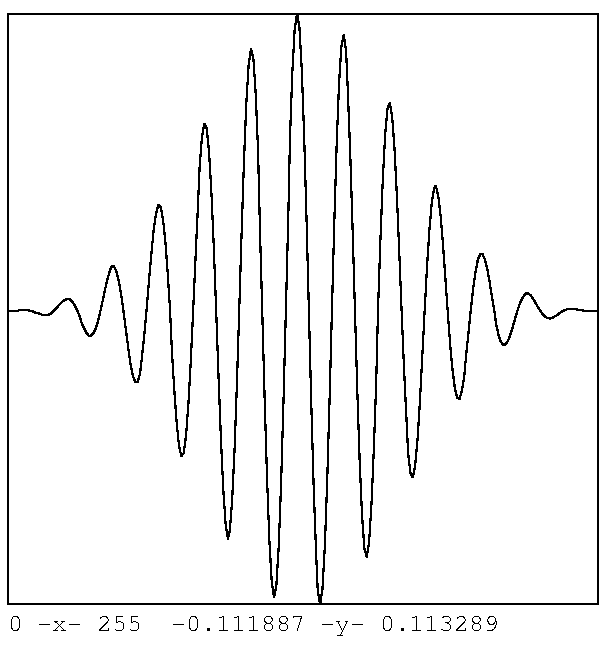
\includegraphics[width=6cm]{fig/window_1.pdf}
\end{center}
\par
This example passes the excitation generated through a train pulse
by a digital filter, applies a Blackman windowing function to it,
evaluates the log magnitude spectrum through 512 points FFT,
and plots the results on the screen:
\begin{quote}
\verb!train -p 50 | dfs -a 1 0.9 | window -l 50 -L 512 |\! \\
\verb!spec -l 512 | fdrw | xgr!
\end{quote}
\begin{center}
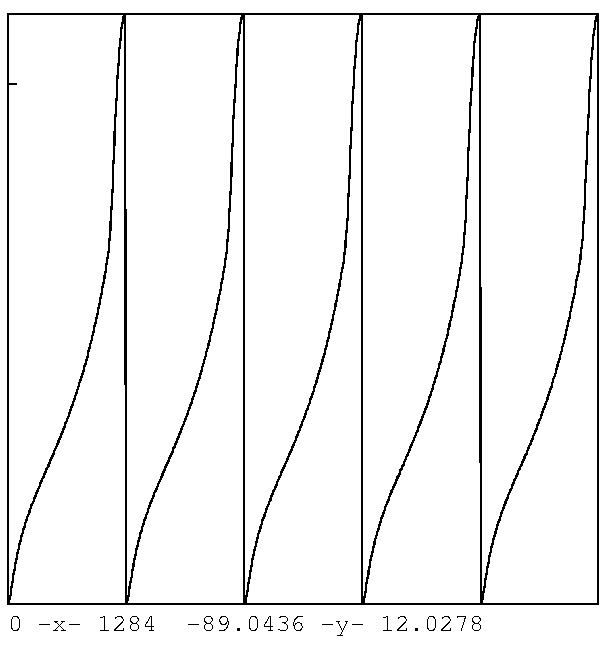
\includegraphics[width=6cm]{fig/window_2.pdf}
\end{center}
\end{qsection}

\begin{qsection}{SEE ALSO}
\hyperlink{fftr}{fftr},
\hyperlink{spec}{spec}
\end{qsection}
